The purpose of this chapter is to benchmark and evaluate memcached performance. Firstly, we will examine performance under default configuration of both the server and the client. Secondly, threading will be explored in relation to latency and throughput. Thirdly, the effect of memcached's \texttt{group size} will be explored in relation to performance. Additionally, configuration of receive and transmit queues will be explored and finally, an execution model of multiple processes will be visited in order to establish a comparison baseline. Throughout the benchmarks, we will be focusing cache performance which meets desired the QoS.


\section{Out of the Box Performance}

Firstly, we consider Memcached in it's default configuration. A list of the configuration parameters as well as the default values is presented in Section \ref{sec:memcached_configuration}. The purpose of benchmarking Memcached in the default configuration is to obtain a baseline performance. This will in turn allow us to consider potential optimizations with respect to the baseline.

The Memcached server is started with the following command.

\begin{lstlisting}
memcached -d -p 11120 -m 6144
\end{lstlisting}

We run Memcached in daemon mode (\textit{-d}), set the maximum amount of memory Memcached can use to 6GB (\textit{-m}) and finally we bind Memcached to port 11120 (textit{-p}). Note that by default, Memcached runs with 4 threads.


In order to generate a workload with increasing intensity, the number of simultaneous connections is increased linearly. As the number of connections grows, so does the number of requests per second issued to Memcached. We configure the Memtier benchmark as follows:

\begin{lstlisting}
  memtier -s <server> -p 11120 -c <connections> -t 3
    --random-data
    --key-minimum=1
    --key-maximum=10000000
    --data-size=32
\end{lstlisting}
Memtier is run simultaneously on 7 hosts (distinct from the server). The Memcached server and port number are provided (\textit{-s}, \textit{-p}). Each host executing Memtier runs 3 distinct threads with \textit{c} connections in each thread. The number of connections increases linearly from 1 connection to 17 connections. As a result, the number of connections in consecutive benchmarks increases by 21. This is the result of running Memtier on 7 hosts with 3 threads per each host. Additionally, the \textit{key-minimum}, \textit{key-maximum} and \textit{data-size} configuration parameters are provided for clarity and are set to the default values configured by Memtier. The result of the above configuration is to generate a linearly increasing load on the Memcached server.


\subsection{Latency, Throughput and Number of Connections}

Firstly, we are interested in the relationship between throughput and latency shown in Figure \ref{fig:memcached-default-latency-vs-ops}. Latency, both mean and 99th percentile, are plotted on the left vertical axis, the number of operations per second is plotted on the right vertical axis and the number of connections used is on the horizontal axis.

\begin{figure}[h]
    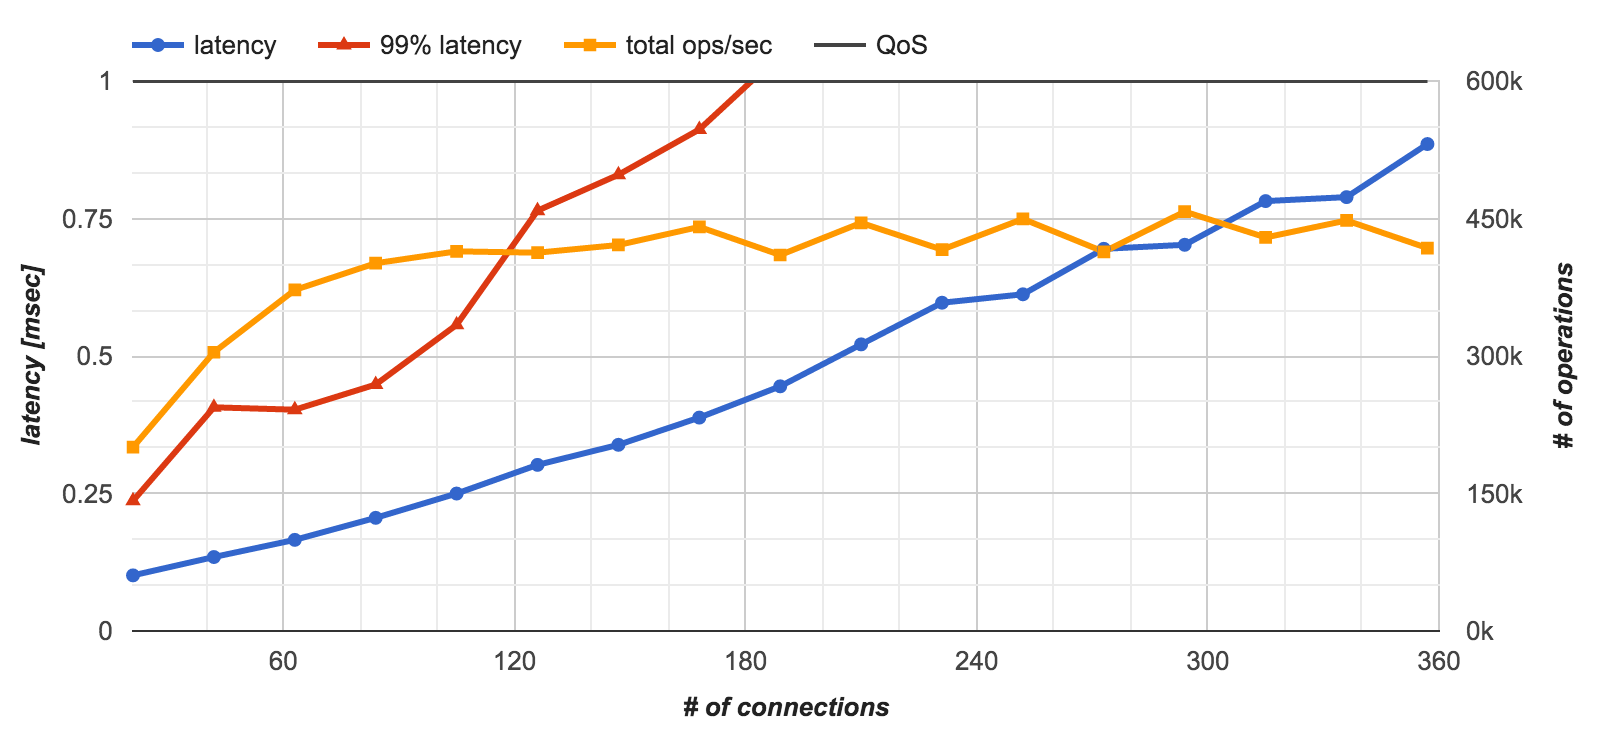
\includegraphics[width=\textwidth]{./res2/m_baseline_latency.png}
    \caption{Latency \& Throughput vs Number of Connections}
    \label{fig:memcached-default-latency-vs-ops}
\end{figure}

As the number of connections increases, mean latency increases too. There is a linear trend between the number of connections and the mean latency. The 99th percentile latency also increases with the number of connections, however, it grows faster than than the number of connections does and exceeds the required QoS constraint at 189 simultaneous connections. The total number of operations, increases quickly as the number of connections increases and begins to flatten at 100 connections or 415k requests per second. As the number of connections increases beyond 100, the throughput remains relatively stable at around 430k requests per second.

Examining the relationship between latency and throughput, we can observe that initially we are able to increase throughput to 415k requests per second, however, a further increase in throughput comes at a disproportionately larger cost in terms of 99th percentile latency. This is reasonable as there is a limit to the number of requests we can process per second, a larger number of requests will incur queuing delay which translates to increased latency.

\subsection{CPU Utilization}

Secondly, we consider the effect of the workload on the Memcached server in terms of CPU Utilization. The CPU utilization is monitored through the \textit{mpstat} \cite{mpstat} utility which reports the percentage of CPU utilization broken down into multiple categories. The following table \cite{mpstat} summarizes the responsibilities of each category.

\begin{enumerate}
    \item [\%usr] Show the percentage of CPU utilization that occurred while executing at the user level (application).
    \item [\%sys] Show the percentage of CPU utilization that occurred while executing at the system level (kernel). Note that this does not include time spent servicing hardware and software interrupts.
    \item [\%iowait] Show the percentage of time that the CPU or CPUs were idle during which the system had an outstanding disk I/O request.
    \item [\%irq] Show the percentage of time spent by the CPU or CPUs to service hardware interrupts.
    \item [\%soft] Show the percentage of time spent by the CPU or CPUs to service software interrupts.
    \item [\%idle] Show the percentage of time that the CPU or CPUs were idle and the system did not have an outstanding disk I/O request.
\end{enumerate}

For the context of this paper, \textit{\%usr} corresponds directly to the CPU utilization used by Memcached as it is the only application running on the server.

Furthermore, \textit{\%soft} represents the software interrupt issued by \textit{libevent} when a new file descriptor is available for processing, that is, a new request is available to be processed or a response is ready to be handed over to the network stack.

\begin{figure}[h]
    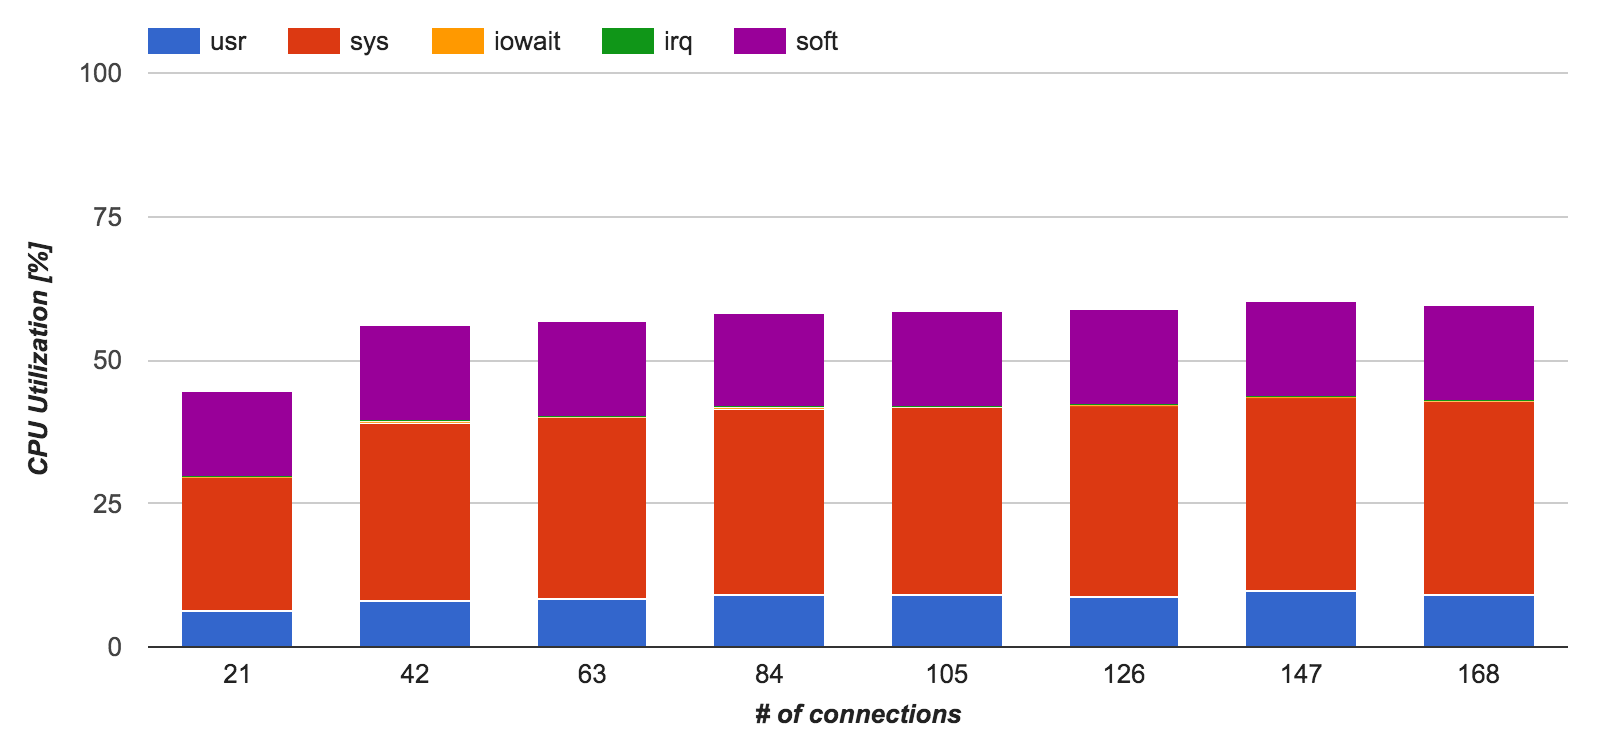
\includegraphics[width=\textwidth]{./res2/m_baseline_cpu.png}
    \caption{CPU Utilization for Out of the Box Configuration of Memcached}
    \label{fig:m_baseline_cpu}
\end{figure}

Figure \ref{fig:m_baseline_cpu} outlines the CPU Utilization broken down into mpstat categories.

Firstly, as the number of connections increases, the \textit{usr} utilization remains nearly constant at 9\%.

Secondly, \texit{sys} utilization increases as the number of connection increases between 21 and 120 connections and remains relatively stable as the number connections increases further. This behavior corresponds to the saturation point also observed in the relationship of connections and throughput.

Thirdly, \textit{soft}, increases as the number of connections increase due to the increased number of requests per second which are required to be serviced.

Finally, \textit{iowait} and \textit{irq} account for less than 0.01\% of the total CPU utilization. This is a reasonable result as Memcached is an in-memory object cache and therefore we do not expect to see any disk I/O.












\subsection{Effect of Connections}
To understand the effect of a large number of connections on the cache performance, Figure \ref{fig:memcached-default_connections} shows the effect an increase in the total number of connections has on throughput, mean latency and the 99th percentile latency. The figure deliberately shows the behavior outside of the requires QoS requirements in order to better illustrate the impact on the cache under high load.

\begin{figure}[h]
    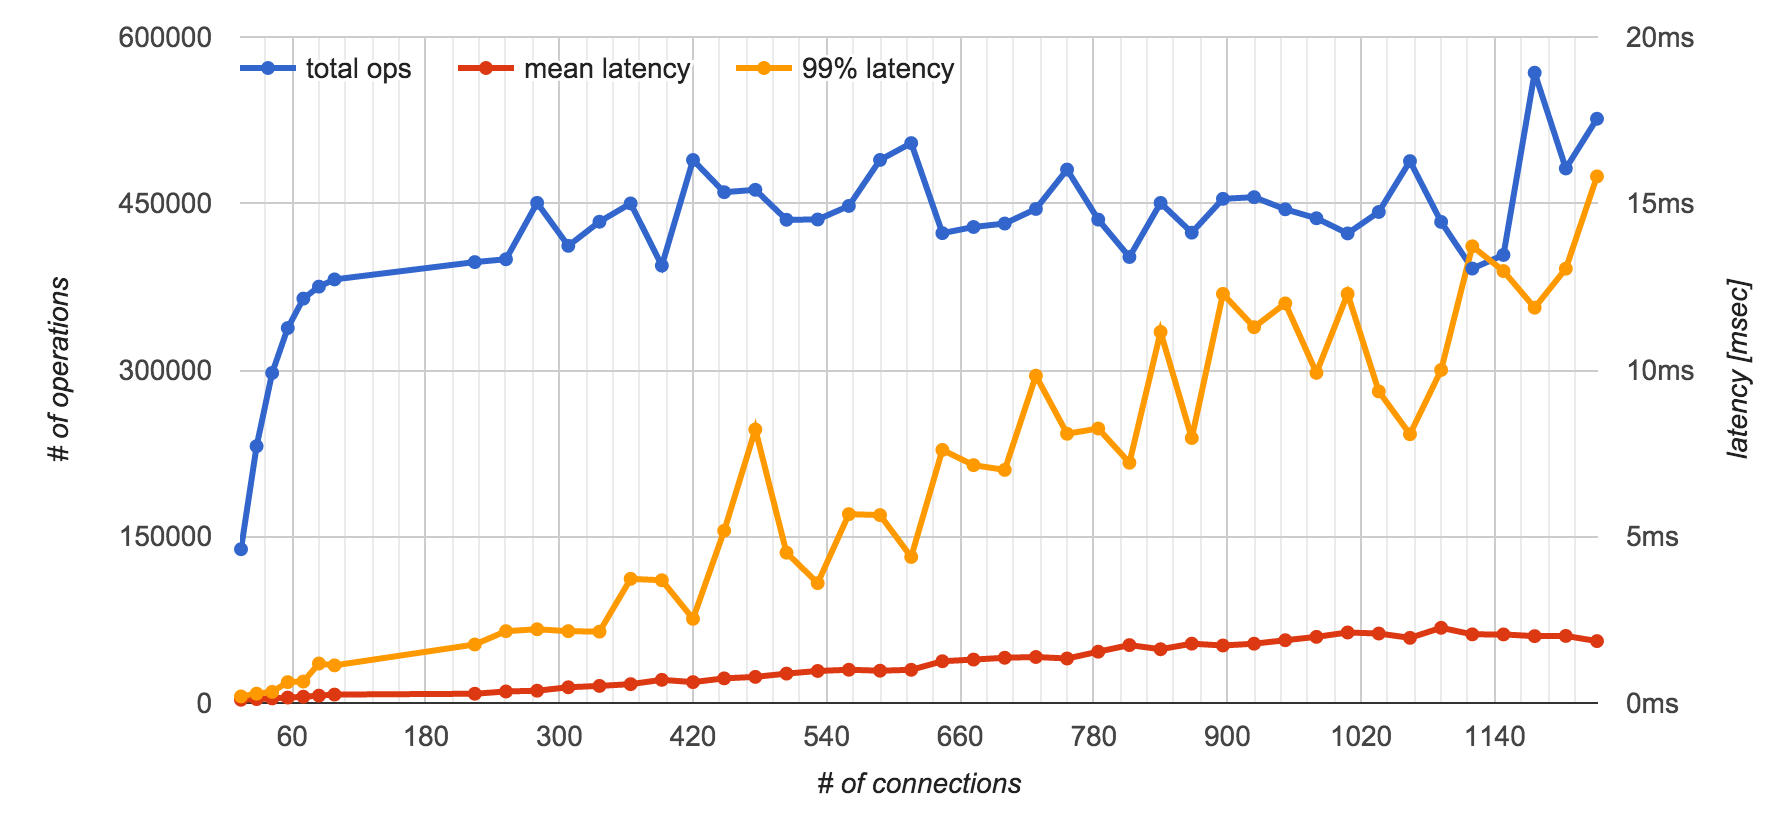
\includegraphics[width=\textwidth]{./res/5_default_connections.png}
    \caption{Throughput, Mean latency and 99th percentile against the number of connections}
    \label{fig:memcached-default_connections}
\end{figure}

Firstly, Figure \ref{fig:memcached-default_connections} displays the general trend an increased load has on throughput. As load increases, so does throughput. However, as the number of connections surpasses 100, the rate of increase in throughput for each increase the number of connections decreases. This is the saturation point of the cache, an increase in load yield disproportionate increase in throughput. Beyond the saturation point, the cache throughput fluctuates around 450,000 operations per second.

Secondly, the mean latency increases linearly with the number of connections (load). This is an expected behavior as the server experiences network stack queuing as well as increased resource requirements to process requests.

Thirdly, the 99th percentile latency increases linearly, with some fluctuations, against the increased server load. As the load gets higher, the fluctuation increases as well as the upper bound. This is due to some requests being queued for a long time before being processed, pushing the 99th percentile high.

We can observe that the server is capable of scaling much better until around 100 connections are reached. When the saturation point is surpassed, overall performance and quality of service degrades.


\subsection{Server CPU}
In order to be better understand the impact of memcached on the system, specifically the CPU usage, we consider a breakdown of CPU time spent in various areas of the operating system in Figure \ref{fig:memcached-default-cpu}.

\begin{figure}[h]
    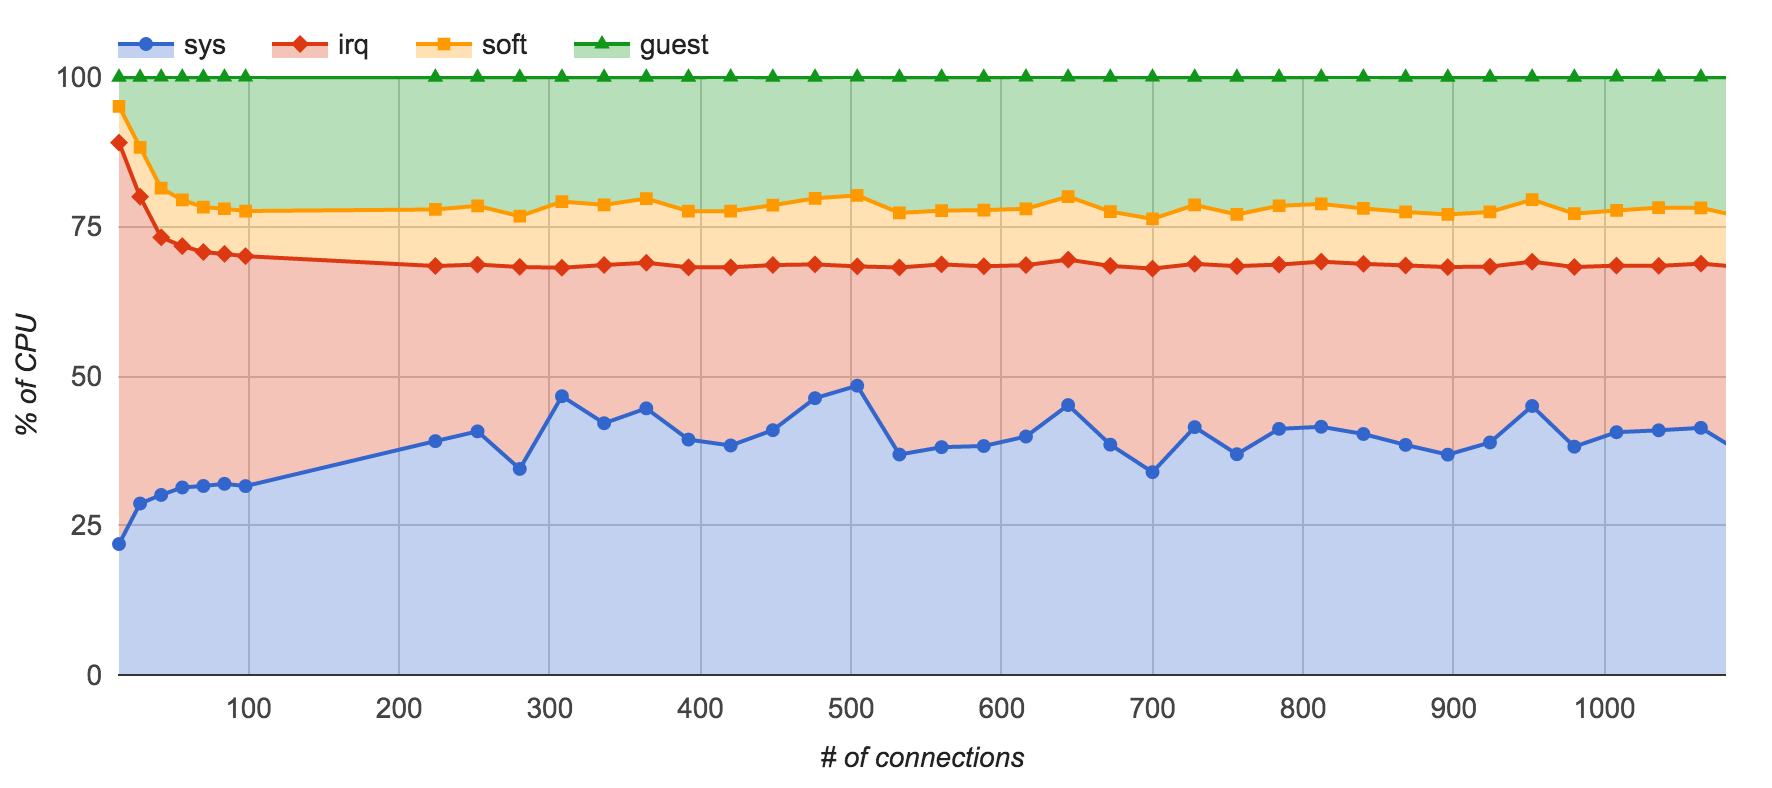
\includegraphics[width=\textwidth]{./res/5_default_cpu.png}
    \caption{CPU Time against number of connections}
    \label{fig:memcached-default-cpu}
\end{figure}

Firstly, we can observe that the effective footprint of memcached (\texttt{guest}) is relatively small compared to the rest. The CPU usage of memcached increases up until 100 connections at which point it remains fairly stable.

Secondly, the operating system (\texttt{sys}) increases as we increase the load. Fluctuations occur past 250 connections but the CPU usage by the system remains around 40 percent as the load is increased further. An increased number of connections requires additional resources to process incoming requests as well as process outgoing requests. The context switching from receiving and transmitting contributes to the high load from the system.

Thirdly, interrupt processing by the system (\texttt{irq}) decreases as we increase load, this is due to having more CPU available and therefore being able to process a higher number of interrupts per unit of time. As resources are required by the system and the memcached application, this number of interrupts processed per unit of time decreases as reflected by the proportion of CPU.

Finally, software interrupt footprint (\texttt{soft}) remains relatively stable throughout. The software interrupts correspond to running threads of the memcached application (4 threads by default) and are used for context switching.

From the breakdown in Figure \ref{fig:memcached-default-cpu}, we can conclude that memcached is not CPU heavy on its own. The large CPU footprint of running memcached under high load is tightly linked to performance of the network stack and the underlying hardware processing network requests rather than the application itself. This observation is consistent with findings in MICA \cite{lim2014mica}.


\section{Memcached Thread Scalability}
Memcached, as a high performance object cache, is designed to be executed on a parallel architecture. It implements scalability through the use multiple threads allowing memcached to utilize many core architectures. Therefore, the next step in scaling a memcached deployment is to provision a larger number of threads for the application.

Memcached execution model is capable of processing incoming and outgoing requests in parallel, however, operations executed require a global application lock to be acquired. Therefore, the expected number of threads maximising throughput while minimizing latency can be expected to be achieved when memcached is provisioned with the same number of threads as hardware CPU cores which is also suggested by Leverich and Kozyrakis \cite{leverich2014reconciling}.

Utilizing findings from the previous section, a configuration with 84 connections can be used to generate a consistent load while the number of threads provisioned for memcached can be varied. Therefore, we can set up each benchmark client as follows:

\begin{lstlisting}
  memtier -s nsl200 -p 11120 -c 6 -t 2 -P memcache_binary
    --random-data
    --key-minimum=100
    --key-maximum=10000
\end{lstlisting}

The server in turn is configured as follows:
\begin{lstlisting}
  memcached -d -p 11120 -m 6144 -t <thread_count>
\end{lstlisting}

Where the number of threads is progressively increased.

\subsection{Throughput \& Latency}

Figure \ref{fig:memcached-threads} shows the relationship between throughput, mean latency and 99th percentile latency in relation to the number of threads used by a memcached application.

\begin{figure}[h]
    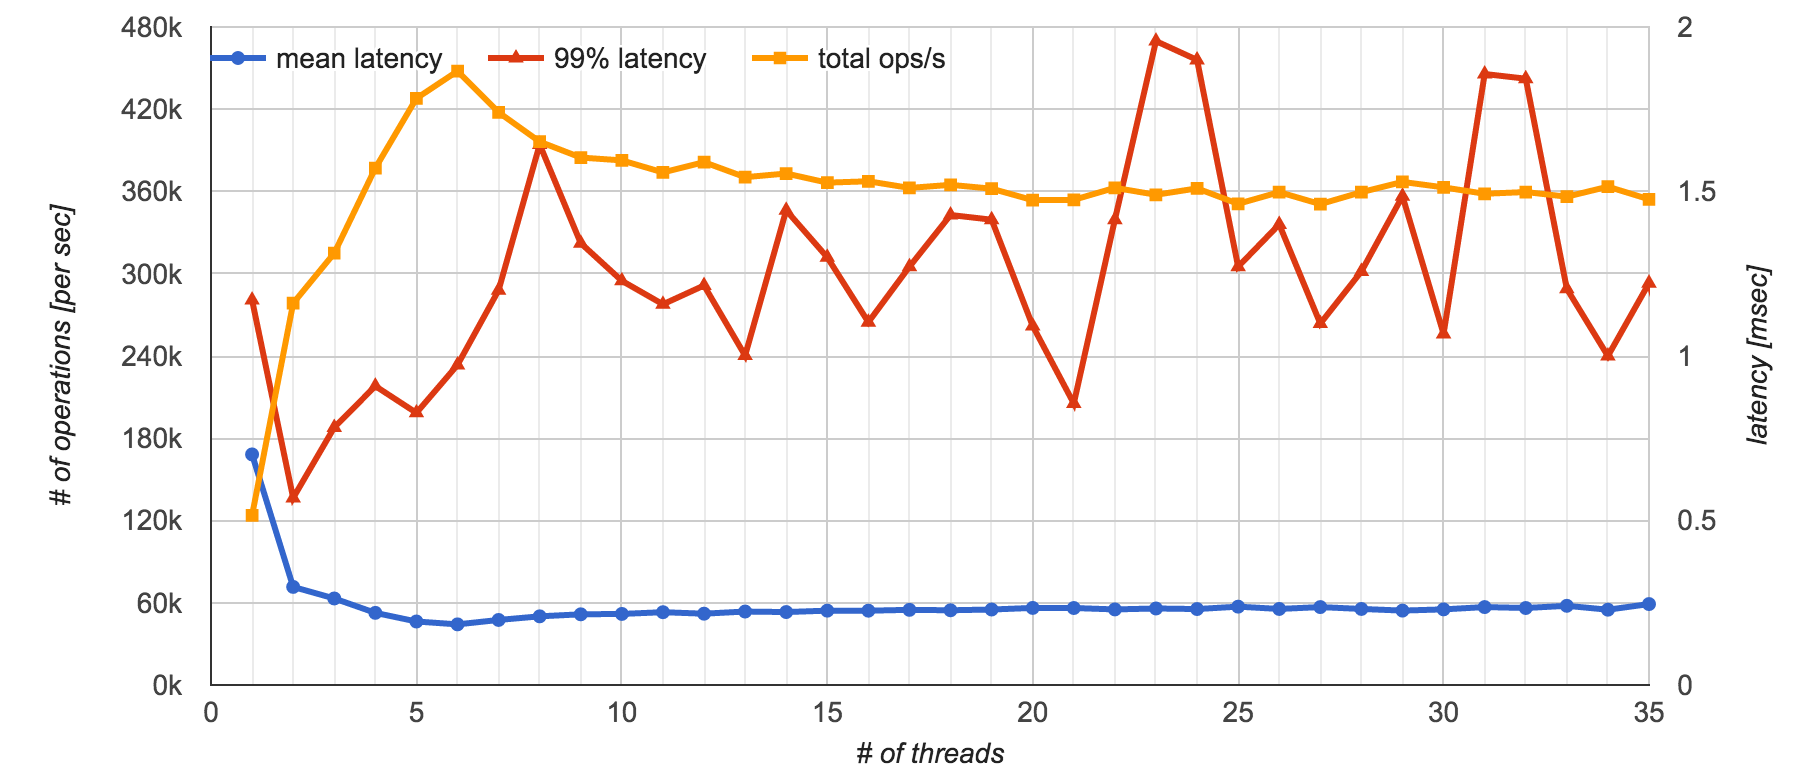
\includegraphics[width=\textwidth]{./res/5_memcached_threads.png}
    \caption{Memcached Thread Scaling}
    \label{fig:memcached-threads}
\end{figure}

Firstly, we can observe that throughput increases as thread count increases until we reach 6 threads where it peaks at 450k requests per second. As we increase thread count further, throughput decreases. This behavior corresponds with our expectation that performance is maximized when there are as many threads as CPU cores.

Secondly, mean latency decreases as the number of threads is increased reaching a minimum of 0.1843 milliseconds at 6 threads. With more threads, the mean latency increases steadily.

Thirdly, the 99th percentile latency decreases as we increase the number of threads from 1 to 2, reaching a minimum and increasing as the number of threads increases. At 6 threads, we reach a 99th percentile latency of 0.973 which satisfies the QoS requirements under 1 millisecond.

Indeed, as expected we have been able to obtain the highest throughput and achieve the quality of service requirements with 6 threads, as many as CPU cores on the host. Beyond 6 threads, the overhead of context switching between threads increases processing time and reduces throughput.

\subsection{CPU Time}

\begin{figure}[h]
    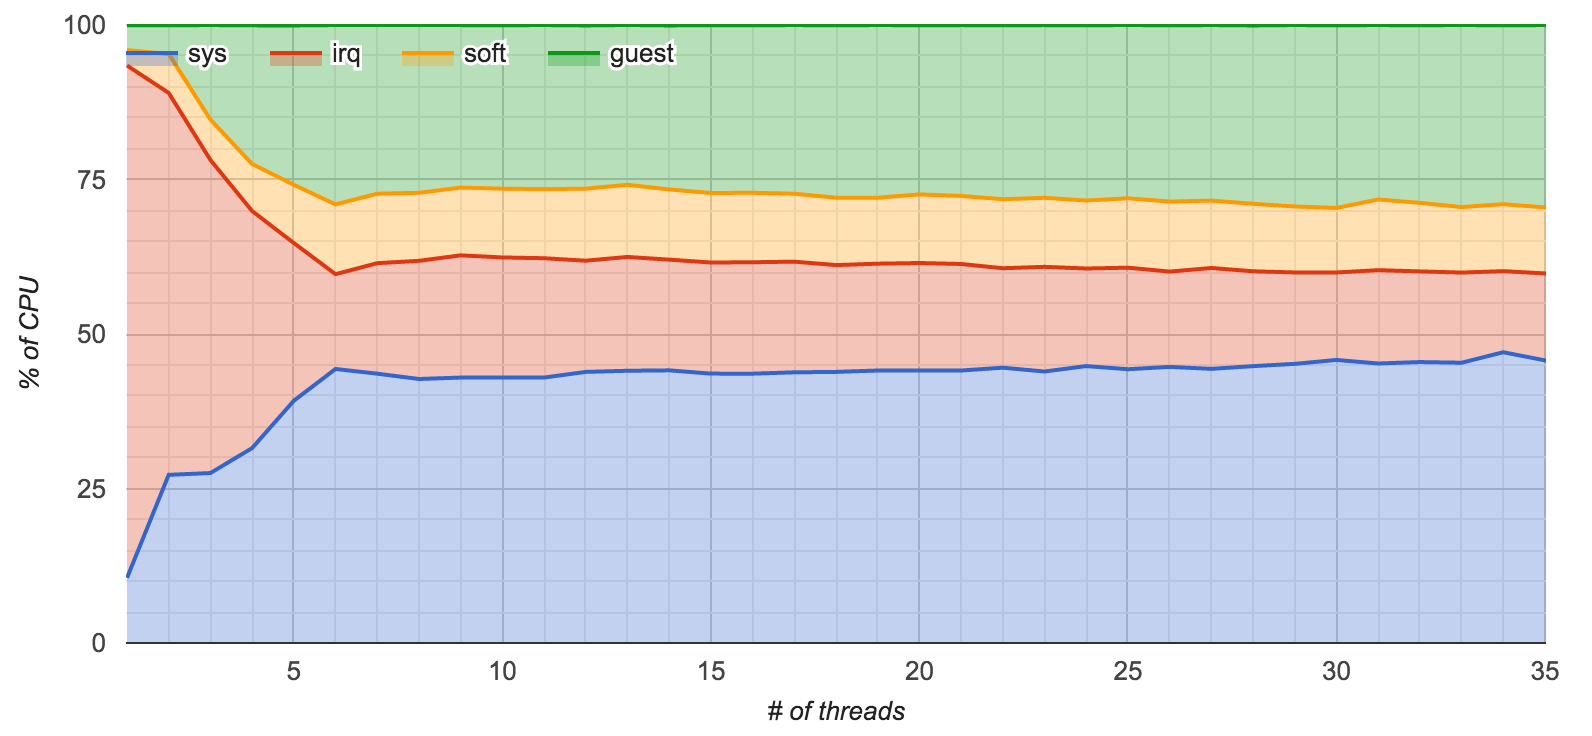
\includegraphics[width=\textwidth]{./res/5_threads_cpu.png}
    \caption{Memcached CPU Time against Number of Threads}
    \label{fig:memcached-threads-cpu}
\end{figure}

Analyzing the CPU usage in Figure \ref{fig:memcached-threads-cpu} as we increase the number of threads, we can observe that initially a large portion of the CPU time is spent servicing hardware interrupts (\textit{irq}). Therefore, the OS is handling incoming traffic interrupts from the NIC. As the number of threads increases, an increasingly larger portion of CPU time is spent processing system calls and context switching (\textit{sys}). This is reasonable as a larger number of threads will require context switching and concurrency management provided by the operating system. We can see that time spent processing hardware interrupts (\textit{irq}) decreases which has the effect of increasing latency as packets remained queued up in the NIC for longer before the OS manages to schedule the interrupt to be serviced. Furthermore, we can observe that software interrupts (\textit{soft}) CPU time progressively increases until we reach 6 threads and remains stable as the number of threads grows further. The initial increase is reasonable as we are demanding more threads to processed simultaneously, past this point the percentage remains stable as we have reached a saturation point in terms of scalability and server performance. Finally, memcached (\textit{guest}) follows a similar pattern as software interrupts. Usage increases until 6 threads are used and saturates further. This is further indicative of the inability to efficiently scale the number of threads past the point at which memcached uses the same number of threads as CPU cores.

\subsection{Thread evaluation}
Comparing results obtain from thread scalability with the results from the default configuration of memcached, we have been able to increase throughput from 375k to 450k requests per second while maintaining the desired QoS under 1ms.



\section{Thread pinning}
\label{sec:thread-pinning}
Thread pinning is the process of assigning a \textit{set\_irq\_affinity} to each individual thread. As suggested by Leverich and Kozyrakis, "pinning memcached threads to distinct cores greatly improves load balance, consequently improving tail latency." \cite{leverich2014reconciling} and therefore the reasonable next step in optimizing memcached performance is to attempt thread pinning and analyse the results obtained.

By default, when a new process is started, its affinity is set to all available CPUs. We can discover a given process affinity by executing the following command where \textit{pid} is the process identifier.

\begin{lstlisting}
    taskset -p <pid>
\end{lstlisting}


"A Memcache instance started with n threads will spawn n + 1 threads of which the first n are worker threads and the last is a maintenance thread used for hash table expansion under high load factor." \cite{solarflarememcached}. We can discover memcached threads used for request processing using the following command where \textit{tid} is the thread id discovered previously \cite{solarflarememcached}.
\begin{lstlisting}
    ps -p <memcache-pid> -o tid= -L | sort -n | tail -n +2 | head -n -1
\end{lstlisting}

Given the best performance under QoS constraints of 1ms found in the previous section is memcached with 6 threads, the following benchmark will be using this best configuration in order the analyze the impact of thread pinning.

\subsection{Throughput vs Latency}

\begin{figure}[h]
    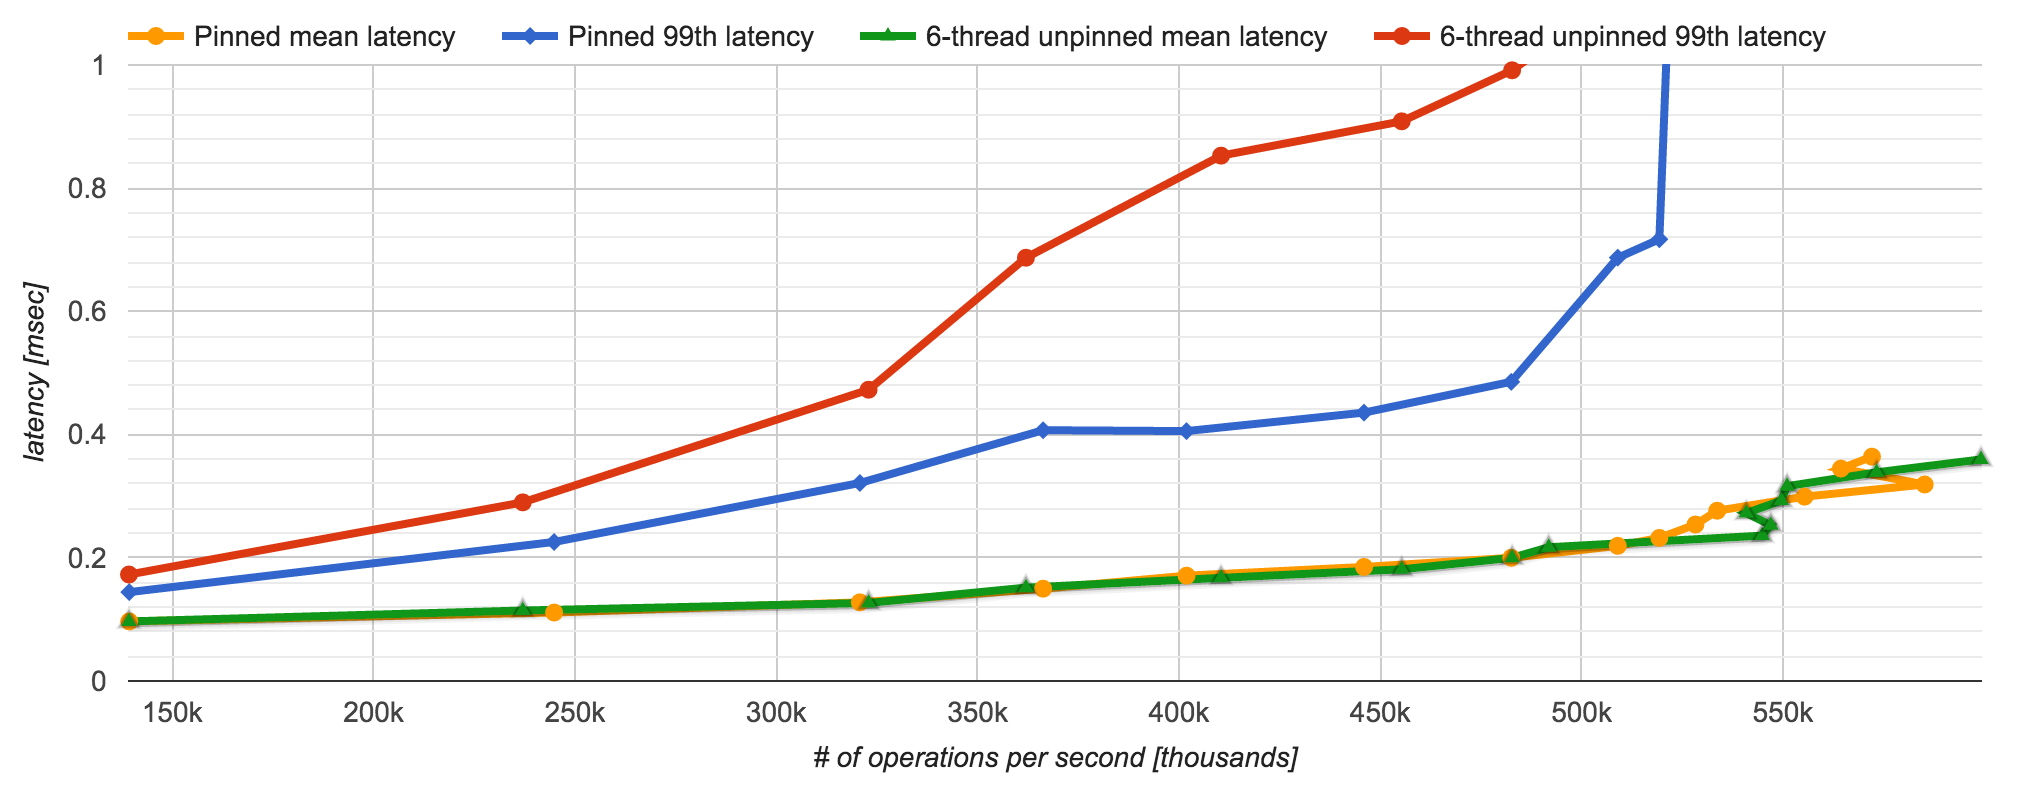
\includegraphics[width=\textwidth]{./res/5_threads_pinned.png}
    \caption{Memcached Pinned Threads vs Unpinned}
    \label{fig:memcached-threads-pinned}
\end{figure}

Figure \ref{fig:memcached-threads-pinned} shows the impact thread pinning has on mean and 99th percentile latency against throughput.

Firstly, the mean latency of both pinned and unpinned benchmarks remains very similar as throughput increases.

Secondly, the 99th percentile latency is lower in the case of pinned threads than unpinned. The pattern holds as throughput increases up until the required QoS boundary.

Furthermore, the throughput has also increased reaching 520k requests per second compared to 475k requests per second in the case of unpinned threads. This pattern is further confirmed by  Leverich and Kozyrakis \cite{leverich2014reconciling}.

The reason for a significant improvement in the tail latency is reduced contention for access to receive and transmission queues in the network stack. Given memcached's design of running \textit{t} threads for request processing and \textit{1} thread for hash table expansion under high load, the result may be two or more request processing threads scheduled on the same CPU core while the hash table expansion thread is scheduled to run alone on a core. Pinning threads prevents this scenario from occurring as well as creates a direct mapping between each receive and transmission queue in the network stack to the memcached thread, reducing need for context switching.


\section{Group Size}
Memcached provides a configuration option \textit{-R} to set the group size used inside memcached. The group size defines the ``Maximum number of requests per event, limits the number of requests process for a given connection to prevent starvation (default: 20)'' \cite{interactive2006memcached}. This in effect means the number of requests that will be processed from a single connection before memcached switches to a different connection to achieve a fair policy.

In order to benchmark the effects of an increased group size, we consider a benchmark scenario where the group size is progressively increased while maintaining a consistent load on the cache. The load used will be the one explored in Section \ref{sec:thread-pinning} - Thread Pinning. All clients will be setup with 2 threads and 9 connections each which corresponds to the best performance under QoS so far. The memcached server will be setup with the \textit{-R} flag set to 20 initially and increased by 20 for each iteration until a maximum (enforced by memcached) of 320 is reached.

\begin{figure}[h]
    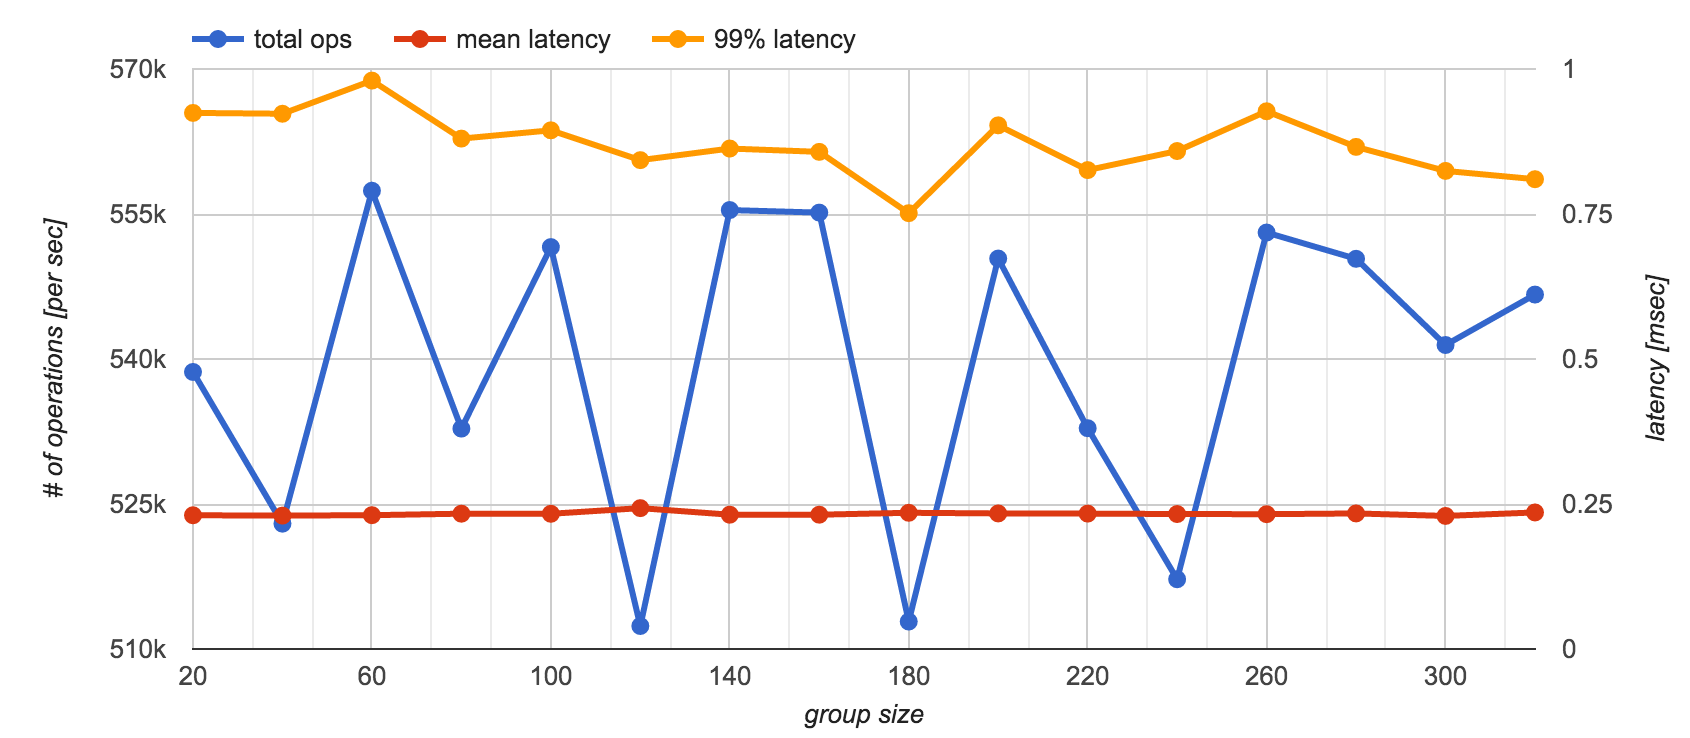
\includegraphics[width=\textwidth]{./res/5_memcached_group_size.png}
    \caption{Memcached Latency, 99th percentile latency and throughput against group size}
    \label{fig:memcached_group_size}
\end{figure}

Figure \ref{fig:memcached_group_size} shows the relationship between throughput, mean latency and 99th percentile latency.

Firstly, we can observe that the throughput achieved fluctuates heavily around 540k requests per second. Secondly, the mean latency remains constant as the group size is increased. Finally, the 99th percentile latency experiences a decreasing trend as group size is increased while staying under the required QoS constraints of 1ms.

By setting \textit{group size} to 320, we have been able to reduce both 99th percentile latency as well as increase the total throughput from 520k to 540k requests per second. Additionally, we have been able to show that the context switching required to achieve a fairness policy of processing only 20 requests from a single connection caused a decrease in performance. Similar results have been obtained by Blake and Saidi \cite{blake54does}. On the other hand, the results observed are dependent on the distributed system model and the expected request rate. In a production environment, benchmarking of a particular workload would show the best configuration in respect to group size.

\section{Receive \& Transmit Queues fixing}
TODO: Haven't been able to obtain any improvements in terms of performance (both throughput and latency), not sure if the topic should still be discussed in detail.


\section{Multiple Memcached Processes}

In this section, we will examine the impact multiple memcached processed have on the overall performance of the caches as a whole. In some applications, it is important to be able to partition the system in such a way systems interact with different instances of memcached. Additionally, this information will also serve as a useful benchmark comparison for Redis performance.